\subsubsection{Skitse af løsning}

\label{sec:skitse_loesning}

\begin{figure}[H]
   \centering
   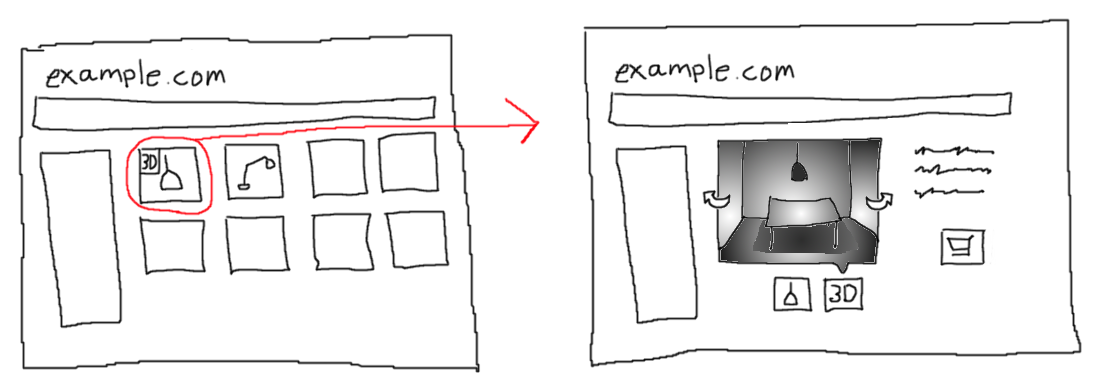
\includegraphics[width=\textwidth]{skitse_til_loesning}
   \caption{Skitse af ide til løsning.}
   \label{fig:skitse_af_ide}
\end{figure}

På figur \ref{fig:skitse_af_ide} er der illusteret en skitse af en e-butik som sælger lamper. Figuren illustrerer hvordan systemet kan integreres på en hjemmeside. Skitse \ref{fig:skitse_af_ide}a viser et online katalog over e-butikkens udvalg af lamper. Som der fremgår af skitsen vil nogle lamper være markeret med et "3D-ikon" og dette indikerer, at kunden har mulighed for, at se skitsen i 3D. Kunden tilgår 3D-billedet ved at klikke på ikonet. Når kunden trykker på ikonet bliver kunden omdirigeret til en anden menu. Som der fremgår af skitse \ref{fig:skitse_af_ide}b, så har kunden her mulighed for at se en \textit{3D-model} af lampen i et rum. De to pile på skitsen indikerer, at kunden har mulighed for at rotere billedet, og se hvordan belysningen fra lampen er, set fra forskellige vinkler. Som en ekstra feature har kunden mulighed for at indtaste en kontekst, beskrevet som en model, ind i programmet og har derefter mulighed for at se hvordan lampen ser ud i den kontekst som kunden ønsker. 
Derudover har kunden mulighed for, at justere lampens farvetemperatur i kelvin, meningen med denne feature er, at kunden har mulighed for at visualisere hvordan forskellige pærer vil se ud i lampen. De forskellige 3D billeder vil ligge til rådighed på en ekstern server og vil derfor ikke gøre e-butikkernes hjemmeside betydeligt langsommere. Derudover er tanken af alle 3D billeder bliver udleveret af producenten af lamperne. 

\begin{figure}[H]
   \centering
   
\includegraphics[width=\textwidth]{brugerinteraktion}
   \caption{Sekvensdiagram af løsningsideen.}
   \label{fig:sekvensdiagram_af_ideen}
\end{figure}

Figur \ref{fig:sekvensdiagram_af_ideen} tager udgangspunkt i en hjemmeside som har fået implementeret vores løsning, og viser et sekvensdiagram som illustrere processen når en kunde vil købe en lampe.  

I forbindelse med implementeringen af softwaren på en hjemmeside har der været forskellige ting som skulle overvejes. Da problemet omhandler visualisering af lys fra lamper, har gruppen valgt at fokusere på at lave en løsning hvis primære formål er at generere realistiske 3D-billeder af lamper. Disse billeder vil vise belysningen fra lamper med forskellige pærer. Features som interaktion og kontekst, har derfor anden priotet. 

